\chapter{Scattering, Mandelstam Variables, and the Open-String Picture}

We begin with a short return to the theme of fermionic strings, but the real subject of this lecture is scattering. That is the natural point of contact between theory and experiment: particles come in, something happens in a collision region, and particles come out. The problem is to encode this process in invariant language, to understand what simple Feynman diagrams would predict, and then to see why the string picture gives a much richer and more symmetric answer than point-particle intuition would have suggested.

\section{From Fermionic Strings Back to Scattering}

Fermionic strings had been introduced to cure two obvious defects of the bosonic theory: they supply fermions and they remove the tachyon. They do not remove the extra dimensions, but at this stage that issue is deliberately deferred. Compactification is named as an important later subject, and then the lecture turns sharply to a more immediate question: how does one compute scattering amplitudes?

The point is practical. Elementary particle physics is largely built out of scattering experiments, not because scattering is the deepest thing that can happen, but because it is what can be measured. We therefore want a mathematical language in which an amplitude can be expressed as a function of the data carried by the incoming and outgoing particles.

\section{Four-Momentum, Mass Shell, and the All-Incoming Trick}

The first step is to isolate the minimal kinematic data. Each particle carries a relativistic four-momentum,
\begin{equation}
K^\mu = (K^0,\vec K),
\end{equation}
with \(K^0\) the energy and \(\vec K\) the spatial momentum. In the lecture the relativistic square is taken in the convention
\begin{equation}
K^2 \equiv \vec K^{\,2} - (K^0)^2.
\end{equation}
The ordinary mass-shell relation is therefore written as
\begin{align}
E^2 &= \vec p^{\,2}+m^2,\\
E^2-\vec p^{\,2} &= m^2,\\
\vec p^{\,2}-E^2 &= -m^2,
\end{align}
so that
\begin{equation}
K^2 = -m^2.
\end{equation}
This is not yet about collisions at all; it is the first invariant statement about a single relativistic particle.

\begin{figure}[htbp]
\centering

\includegraphics[width=0.72\textwidth]{lecture_06_figure_02.png}

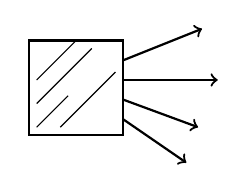
\begin{tikzpicture}[scale=1.0]
\draw[thick] (0,0) rectangle (1.2,1.2);
\draw (0.1,0.1) -- (0.5,0.5);
\draw (0.1,0.4) -- (0.8,1.1);
\draw (0.1,0.7) -- (0.6,1.2);
\draw (0.4,0.1) -- (1.1,0.8);
\draw[->,thick] (1.2,0.95) -- (2.2,1.35);
\draw[->,thick] (1.2,0.70) -- (2.4,0.70);
\draw[->,thick] (1.2,0.45) -- (2.15,0.10);
\draw[->,thick] (1.2,0.20) -- (2.00,-0.35);
\end{tikzpicture}
\caption{The lecture begins the scattering discussion with a black-box collision picture. The screenshot preserves the board transition into four-momentum notation; the accompanying sketch simply cleans up the outgoing-arrow geometry without inventing the unfinished formula on the board.}
\end{figure}

For a \(2\to2\) process, if the outgoing momenta are called \(Q_3\) and \(Q_4\), ordinary energy-momentum conservation says
\begin{equation}
K_1+K_2 = Q_3+Q_4.
\end{equation}
Susskind then uses a standard and very useful trick: redefine the outgoing momenta with a minus sign and treat all legs as incoming,
\begin{equation}
K_3=-Q_3,\qquad K_4=-Q_4.
\end{equation}
Then conservation becomes
\begin{equation}
K_1+K_2+K_3+K_4=0.
\end{equation}
The point of the trick is symmetry. The process can now be discussed as if it involved four incoming momenta subject only to the overall constraint above and to the on-shell condition \(K_i^2=-m_i^2\) for each leg.

The scattering amplitude is then some function
\begin{equation}
A=A(k_1,k_2,k_3,k_4),
\end{equation}
but it cannot really depend on all components independently, because the momenta are constrained.

\section{Center-of-Mass Kinematics and Mandelstam Variables}

At first sight the amplitude seems to depend on many variables. But for two-body scattering the physical content is much smaller. One can always pass to the center-of-mass frame, where the incoming spatial momenta are equal and opposite, and then rotate axes so that the collision lies along a convenient direction. For identical external masses, once this is done, the process is characterized only by the total center-of-mass energy and the scattering angle.

The lecture then looks for relativistically invariant combinations that encode exactly this reduced information. With the all-incoming convention, we define
\begin{equation}
(k_1+k_2)^2=-s,\qquad (k_1+k_3)^2=-t,\qquad (k_1+k_4)^2=-u.
\end{equation}
These are the Mandelstam variables, written in a way compatible with the lecture's sign convention for \(K^2\).

The first of these has an immediate interpretation. In the center-of-mass frame,
\begin{align}
(k_1+k_2)^2
&= (\vec k_1+\vec k_2)^2-(k_1^0+k_2^0)^2\\
&= -E_{\mathrm{cm}}^2,
\end{align}
because the spatial parts cancel. Thus
\begin{equation}
s=E_{\mathrm{cm}}^2.
\end{equation}

The second invariant is the momentum transfer. Since \(k_3=-q_3\),
\begin{equation}
(k_1+k_3)^2=(k_1-q_3)^2.
\end{equation}
In the center-of-mass frame, if \(|\vec p|\) is the magnitude of either incoming spatial momentum and \(\theta\) is the deflection angle, then in the cleaned convention one has
\begin{equation}
-t = 2|\vec p|^2(1-\cos\theta),\qquad -u = 2|\vec p|^2(1+\cos\theta).
\end{equation}
These formulas should be read as the standard reconstruction of the relation that Susskind describes verbally several times: \(t\) measures momentum transfer and therefore knows about the scattering angle.

\subsection{Question \& Answer}

Question. If the scattering depends only on energy and angle, why do we suddenly have three variables \(s,t,u\)?

Answer. Because \(s,t,u\) are not independent. Using
\begin{equation}
k_1+k_2+k_3+k_4=0
\end{equation}
together with the on-shell conditions \(k_i^2=-m^2\) for equal external masses, one finds
\begin{equation}
s+t+u=4m^2.
\end{equation}
So three symmetric invariants have been introduced, but only two independent combinations remain. That is exactly what the center-of-mass analysis told us should happen.

\section{Channel Diagrams, Direct and Crossed}

Once the invariants have been identified, one can attach them to simple Feynman diagrams. In the direct process, particles \(1\) and \(2\) coalesce into an intermediate state of mass \(M\), which later decays into \(3\) and \(4\). The amplitude has the schematic form
\begin{equation}
A_s \sim \frac{g^2}{s-M^2}.
\end{equation}
This is the \(s\)-channel. It depends only on the center-of-mass energy. In the most naive picture it does not remember the incident direction, so it tends to treat different scattering angles democratically.

\begin{figure}[htbp]
\centering

\includegraphics[width=0.62\textwidth]{lecture_06_figure_03.png}

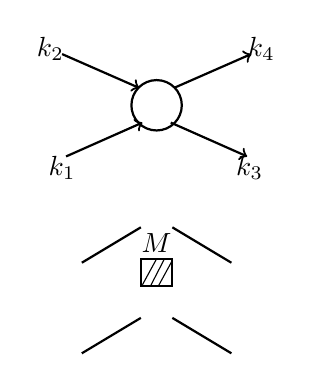
\begin{tikzpicture}[scale=1.0]
\draw[thick] (0,1.8) circle (0.32);
\draw[->,thick] (-1.2,2.45) -- (-0.22,2.02);
\draw[->,thick] (-1.15,1.15) -- (-0.18,1.58);
\draw[->,thick] (0.22,2.02) -- (1.20,2.45);
\draw[->,thick] (0.18,1.58) -- (1.15,1.15);
\node at (-1.35,2.52) {$k_2$};
\node at (-1.20,1.00) {$k_1$};
\node at (1.33,2.52) {$k_4$};
\node at (1.18,1.00) {$k_3$};

\draw[thick] (-0.95,-0.2) -- (-0.20,0.25);
\draw[thick] (-0.95,-1.35) -- (-0.20,-0.90);
\draw[thick] (0.20,0.25) -- (0.95,-0.2);
\draw[thick] (0.20,-0.90) -- (0.95,-1.35);
\draw[thick] (-0.20,-0.50) rectangle (0.20,-0.15);
\draw (-0.18,-0.48) -- (0.00,-0.15);
\draw (-0.08,-0.50) -- (0.10,-0.15);
\draw (0.02,-0.50) -- (0.20,-0.17);
\node at (0,0.05) {$M$};
\end{tikzpicture}
\caption{The board layout for the direct and crossed channels. The upper sketch shows the four external momenta meeting at a single interaction point; the lower sketch isolates the intermediate state of mass \(M\) in the alternate channel.}
\end{figure}

There is also the crossed process, in which the relevant invariant is \(t\). One writes
\begin{equation}
A_t \sim \frac{g^2}{t-M^2}.
\end{equation}
This is the \(t\)-channel. Here the amplitude depends on momentum transfer, so it is angle-dependent from the start. The lecture emphasizes the physical contrast: in the direct channel a compound state is formed and later decays, while in the crossed channel one thinks instead of exchange.

A third possibility,
\begin{equation}
A_u \sim \frac{g^2}{u-M^2},
\end{equation}
is also present in principle, although Susskind does not linger on its diagram because it is awkward to draw cleanly on the blackboard.

\section{The Veneziano Puzzle}

These simple pole formulas are too crude to describe meson scattering. The reason is easy to state: there are many possible intermediate states, not just one. The collision can excite whole towers of particles with different masses and angular momenta. One might therefore try to sum many \(s\)-channel contributions, many \(t\)-channel contributions, and so on.

Historically, however, a remarkable formula appeared that seemed already to know about all of this structure at once. In cleaned modern notation one may write the Veneziano amplitude as
\begin{equation}
A_{\mathrm V}(s,t)\propto B(-s,-t)=\frac{\Gamma(-s)\Gamma(-t)}{\Gamma(-s-t)}.
\end{equation}
Susskind does not dwell on gamma-function technology itself. The point is conceptual: this amplitude has the right pole structure to look like a tower in the \(s\)-channel, but because it is symmetric in \(s\) and \(t\), it also looks like a tower in the crossed channel.

\subsection{Question \& Answer}

Question. How can one amplitude replace separate \(s\)-channel and \(t\)-channel sums without adding them by hand?

Answer. That is exactly the mystery that led people toward string theory. The Veneziano amplitude behaves as though the direct-channel and crossed-channel descriptions are not separate contributions that must be appended, but two readings of a deeper single object. In the lecture, that deeper object is about to become the worldsheet of a string interaction.

\section{Open Strings, Worldsheets, and the Wave Equation}

Susskind now explicitly rewinds from the amplitude back to the mechanism that produces it. We begin with an open string parameterized by
\begin{equation}
0\le \sigma\le \pi.
\end{equation}
The parameter \(\sigma\) is not a spacetime coordinate; it merely labels points along the string. As time evolves, the string sweeps out a strip, and the old world line of a point particle becomes a worldsheet.

\begin{figure}[htbp]
\centering

\includegraphics[width=0.78\textwidth]{lecture_06_figure_04.png}

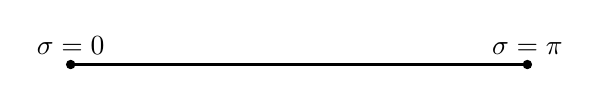
\begin{tikzpicture}[scale=1.0]
\draw[thick] (0,0) -- (5.8,0);
\fill (0,0) circle (0.06);
\fill (5.8,0) circle (0.06);
\node[above] at (0,0) {$\sigma=0$};
\node[above] at (5.8,0) {$\sigma=\pi$};
\end{tikzpicture}
\caption{The open-string parameter interval. The board image records the moment when the endpoints are being labeled; the clean interval below supplies the endpoint labels that the lecture describes explicitly.}
\end{figure}

Each point on the worldsheet is labeled by \((\sigma,\tau)\), where \(\tau\) is the worldsheet time. The embedding of the string into spacetime is described by a coordinate \(X(\sigma,\tau)\). The equation of motion is the wave equation along the strip,
\begin{equation}
\frac{\partial^2 X}{\partial \tau^2}-\frac{\partial^2 X}{\partial \sigma^2}=0.
\end{equation}

\begin{figure}[htbp]
\centering

\includegraphics[width=0.62\textwidth]{lecture_06_figure_05.png}
\caption{The worldsheet wave equation as written on the board. The variable is written simply as \(X\), and that notation is preserved here.}
\end{figure}

At this stage the lecture becomes deliberately concrete. Rather than working directly in the continuum, one imagines the string as a large collection of mass points connected by springs. In that language the worldsheet becomes a collection of nearby world lines, and the dynamics becomes a large coupled system of harmonic oscillators. This is precisely the sort of system we know how to quantize.

\section{Two Strings Coalesce, Evolve, and Separate Again}

We now come to the operational construction of the string scattering amplitude. Consider two incoming open strings, each represented as a chain of \(n\) points. For the first chain, the center-of-mass position is
\begin{equation}
X_{\mathrm{cm}}^{(1)}=\frac{x_1+\cdots+x_n}{n},
\end{equation}
and similarly for the second chain,
\begin{equation}
X_{\mathrm{cm}}^{(2)}=\frac{x_{n+1}+\cdots+x_{2n}}{n}.
\end{equation}
The incoming state is the product of two single-string wavefunctions,
\begin{equation}
\Psi_{\mathrm{in}}
=
e^{ik_1\cdot X_{\mathrm{cm}}^{(1)}}\psi_0(x_1,\dots,x_n)\,
e^{ik_2\cdot X_{\mathrm{cm}}^{(2)}}\psi_0(x_{n+1},\dots,x_{2n}).
\end{equation}
The plane-wave factors encode the center-of-mass momenta \(k_1\) and \(k_2\); the functions \(\psi_0\) encode the internal ground states of the two strings.

The interaction begins by imposing the endpoint coincidence condition
\begin{equation}
x_n=x_{n+1}.
\end{equation}
That picks out the piece of the incoming wavefunction in which the endpoint of one string touches the endpoint of the other. At that moment the two strings are allowed to coalesce into a single longer chain. One then evolves this joined state forward for some interval of worldsheet time, which the lecture again calls \(\tau\). In cleaned notation the update rule is
\begin{equation}
\Psi(\tau)=e^{-iH\tau}\Psi(0),
\end{equation}
where \(H\) is the Hamiltonian of the joined chain of oscillators.

The final step is to project the evolved state back onto a two-string outgoing state with momenta \(k_3\) and \(k_4\). The lecture is explicit about the logical order:
\begin{enumerate}
\item start with two incoming strings,
\item constrain the endpoints to coincide,
\item evolve the joined system as a single string,
\item project onto a separated final state.
\end{enumerate}
What remains is to sum over the possible duration of the intermediate joined state.

\subsection{Question \& Answer}

Question. Why do we integrate over the intermediate time \(\tau\)?

Answer. Because in this setup the lifetime of the compound string is the remaining continuous parameter, and Feynman's rule is to sum over all possibilities. Here that means integrating over every possible duration for which the joined string exists before it splits again.

With the signs cleaned into a consistent convention, the amplitude takes the schematic form
\begin{equation}
A(s,t)\propto \int_0^\infty d\tau\, e^{-\tau(s+1)}\bigl(1-e^{-\tau}\bigr)^{-t-1}.
\end{equation}
The lecture arrives at this formula with several live corrections of signs and exponential factors, so it should be read as the stabilized version of that discussion rather than as a verbatim blackboard transcription.

Now make the change of variables
\begin{equation}
z=e^{-\tau}.
\end{equation}
Since \(\tau=0\) corresponds to \(z=1\) and \(\tau\to\infty\) corresponds to \(z\to0\), the integral becomes
\begin{equation}
A(s,t)\propto \int_0^1 z^{-s-1}(1-z)^{-t-1}\,dz.
\end{equation}
This is the Euler beta function,
\begin{equation}
A(s,t)\propto B(-s,-t)=\frac{\Gamma(-s)\Gamma(-t)}{\Gamma(-s-t)}.
\end{equation}
So the string joining-and-splitting picture reproduces precisely the kind of amplitude that had seemed so mysterious in the older hadronic models.

\subsection{Question \& Answer}

Question. In the discrete string picture, when two endpoint constituents meet, why do two disappear rather than one?

Answer. The lecture treats this as a heuristic but important consistency check. One should think of the touching endpoint of the first chain and the touching endpoint of the second chain as annihilating as a pair, so that the new spring connects the next surviving constituents. In that discrete language the joined chain has \(2n-2\) constituents rather than \(2n-1\). For the continuum limit this distinction is negligible in size, but conceptually it matters, especially if one wants to avoid losing an odd number of fermionic degrees of freedom.

The lecture then briefly notes that the same logic applies, with only slight modifications, to bosonic strings, superstrings, and also to closed strings. The kinematic output is similar, but the deeper explanation of the \(s\)-\(t\) symmetry is still pending.

\section{Summary}

The lecture builds a remarkably tight chain of ideas. We start with ordinary relativistic scattering, reduce the kinematics to invariant data, and package that data into the Mandelstam variables. Simple point-particle diagrams then suggest distinct direct and crossed channels, but the Veneziano amplitude refuses to behave like a mere sum of separate channels. The string picture resolves the puzzle by replacing the point-particle event with a worldsheet process in which two strings join, propagate as one, and split again.

What emerges is not merely a historical curiosity. The amplitude is calculable because the joined string is, in the end, a large system of harmonic oscillators, and the result is symmetric in \(s\) and \(t\) in a way that point-particle intuition had not anticipated. The lecture ends by postponing the deeper reason for that symmetry: conformal symmetry on the worldsheet, which will allow the same process to be read in more than one channel without contradiction.